\chapter{Technical work}
\label{CHAPTER:TechnicalWork}

\glsresetall % Resetting all acronyms

%Status: DONE

The author as member of the \gls{CMS} collaboration was required like all other members perform service work in order to become member of the \gls{CMS} author list. This has been fulfilled with work for the \gls{L1T} system. This work had a field work component in the form of Trigger and Shift Leader shifts in the experiment control room and on call shifts as the Trigger \gls{DOC} expert. Another important component was work as a software developer for the \gls{L1T} \gls{DQM} system. The authors contributions lead his appointment for two years  to the position of coordinator of the software development of the \gls{CMS} \gls{L1T} \gls{DQM} team. This chapter describes the tools developed and used for online monitoring of the \gls{L1T} during 2012-13 data taking as well as for data certification for physics use.

%%%%%%%%%%%%%%%%%%%%%%%%%%%%%%%%%%%%%%%%%%%%%%%%%%%%%%%%%%%%%%%%%%%%%%%%%%%%%%%%%%%%%%%
%%% SECTION
%%%%%%%%%%%%%%%%%%%%%%%%%%%%%%%%%%%%%%%%%%%%%%%%%%%%%%%%%%%%%%%%%%%%%%%%%%%%%%%%%%%%%%%
\section{Data Quality Monitoring}
\label{SECTION:TechnicalWork_DataQualityMonitoring}

%Status: DONE

The \acrfull{DQM} is a critical monitoring system that has an important role in detector and operations efficiency, and certification of recorded data for physics analysis \cite{CMSTDR:CMSTridasTDRVol1,ARTICLE:CMSDataQualityMonitoringSoftWare_ExperienceAndFuture}. The \gls{DQM} system is an end-to-end solution that provides tools to create, fill, display and archive histograms and scalar monitors. It provided the ability to monitor the detector and \gls{DAQ} in real-time, analyse the reconstruction process, validate the experiment software releases and its simulated data. The purpose of this system is to identify problems or errors in both hardware and software as early and accurately as possible.

%%%%%%%%%%%%%%%%%%%%%%%%%%%%%%%%%%%%%%%%%%%%%%%%%%%%%%%%%%%%%%%%%%%%%%%%%%%%%%%%%%%%%%%
%%% SUBSECTION
%%%%%%%%%%%%%%%%%%%%%%%%%%%%%%%%%%%%%%%%%%%%%%%%%%%%%%%%%%%%%%%%%%%%%%%%%%%%%%%%%%%%%%%
\subsection{Online Monitoring}
\label{SECTION:TechnicalWork_DataQualityMonitoring_OnlineMonitoring}

%Status: DONE

The online \gls{DQM} system is composed of several applications that are part of the \gls{CMS} data processing work flow. The software is execute at the \gls{CMS} point 5 computing cluster and applications fall into two categories: \textit{high level trigger modules} and \textit{data quality monitoring modules}. The \textit{high level trigger modules} are run directly in the \gls{HLT} filter farm and can only produce a limited number of histograms with the purpose of monitoring this system or specific \gls{HLT} path. The \textit{data quality monitoring modules} run on a dedicated \gls{DQM} event stream with a rate of $5-10\,\hertz$. These events contain the raw detector and trigger information. Each subsystem has its own application which can analyse all events from the stream or filter a subset with a predefined trigger selection. At the end of every luminosity section, which corresponds to $23.31\,\second$, histograms are gathered from the nodes where the applications are running and merged. The results are showed in real time in a web based application which is accessible by the shift crew and on call experts.

%%%%%%%%%%%%%%%%%%%%%%%%%%%%%%%%%%%%%%%%%%%%%%%%%%%%%%%%%%%%%%%%%%%%%%%%%%%%%%%%%%%%%%%
%%% SUBSECTION
%%%%%%%%%%%%%%%%%%%%%%%%%%%%%%%%%%%%%%%%%%%%%%%%%%%%%%%%%%%%%%%%%%%%%%%%%%%%%%%%%%%%%%%
\subsection{Offline Monitoring}
\label{SECTION:TechnicalWork_DataQualityMonitoring_OfflineMonitoring}

%Status: DONE

The offline \gls{DQM} is used in numerous workflows including monitoring of the event reconstruction process, alignment and calibration validation, \gls{CMS} software release validation, etc. For all this task a standardized two step process is run. 

In the first step histograms are produced in the same computing jobs of the task to be monitored and stored along with the rest of the event data. This is happens in multiple simultaneous jobs which depending on the task can be at Tier 0 or Tier 1 level.

In the second \textit{harvesting step}, the histograms are extracted from the event data and summed together. The resulting histograms contain the full event yields from each run for each processed dataset. Application running at the step have access to the detector conditions from \gls{DCS} and \gls{DAQ} conditions and can produce new histograms such as summaries of the relevant quantities for each run.

%%%%%%%%%%%%%%%%%%%%%%%%%%%%%%%%%%%%%%%%%%%%%%%%%%%%%%%%%%%%%%%%%%%%%%%%%%%%%%%%%%%%%%%
%%% SECTION
%%%%%%%%%%%%%%%%%%%%%%%%%%%%%%%%%%%%%%%%%%%%%%%%%%%%%%%%%%%%%%%%%%%%%%%%%%%%%%%%%%%%%%%
\section{Level 1 Trigger Data Quality Monitoring}
\label{SECTION:TechnicalWork_L1TDQM}

%Status: Writting

The \acrfull{L1T} \acrfull{DQM} is composed of four applications. The first two application run as a part of the online \gls{DQM} system with the mission of monitoring the trigger and trigger emulation in real-time. The second pair of application runs in the offline \gls{DQM} system as part of the (re-)reconstruction workflow with the main function of providing information for physics data certification.

First of the two online applications directly monitors the operation of the trigger. Each trigger subsystem produces plots over the produced objects or relevant quantities which allow to pin-point the origin of problems. Additionally, global trigger operation is monitored in key aspect such as the value of reference algorithm rates, synchronization of firing, finding regions of the detector that fires with unexpectedly high/low rate. The second online application compares the results of the trigger against a real-time software emulation of the system which should allow quick detection of trigger miss configuration or degradation of quality of operation.

Both offline monitoring applications replicate the analysis preformed by their online counterparts but over a the complete recorded dataset for each run.

In the next sections we will focus only on the trigger monitoring tools that the author developed or improved.

%%%%%%%%%%%%%%%%%%%%%%%%%%%%%%%%%%%%%%%%%%%%%%%%%%%%%%%%%%%%%%%%%%%%%%%%%%%%%%%%%%%%%%%
%%% SUBSECTION
%%%%%%%%%%%%%%%%%%%%%%%%%%%%%%%%%%%%%%%%%%%%%%%%%%%%%%%%%%%%%%%%%%%%%%%%%%%%%%%%%%%%%%%
\subsection{Rates Monitoring}
\label{SECTION:TechnicalWork_L1TDQM_RatesMonitoring}

%Status: DONE

The rates monitoring tool has the objective of inspecting the firing rate of each \gls{L1T} object category. At the beginning of each run the \gls{L1T} menus is analysed and for each object category the lowest thresholds unprescaled algorithm is selected. If no unprescaled algorithm is available the lowest prescale and threshold trigger is selected. If the selected trigger algorithms are $\eta$ restricted a warning is showed in the produced histograms to identify that the test performed do not cover the full acceptance of the monitored object. The following categories of objects can be monitored: Electron-Gamma, Isolated Electron-Gamma, Central Jets ($|\eta|<3$), Forward Jets ($3<|\eta|<5$), All Jets ($|\eta|<5$), Taus, Muon, total energy (ETT), total energy in jets (HTT), missing energy (ETM) and jets missing energy (HTM).

When the algorithms to be monitored are determined the tool retrieves from an external database the expected algorithm cross section as a function of instantaneous luminosity. This function are updated daily by fitting runs from the previous days with similar condition. This task is executed by the \gls{WbM} which is a \gls{CMS} monitoring system which runs in parallel to the \gls{DQM}. The algorithm cross section for each luminosity section calculated is calculated with following equation \ref{EQUATION:TechnicalWork_AlgoCrossSection}.

\begin{equation}
\sigma_{\text{Algo}}=\frac{\text{Prescale}_{\text{Algo}}*{\text{Avg. Rate}_{\text{Algo}}}}{\text{Avg. Instantaneous Luminosity}*(1-\text{CMS Dead time fraction})}
\label{EQUATION:TechnicalWork_AlgoCrossSection}
\end{equation}

For each luminosity section the measured value is compared with prediction from previous runs. The monitor presents this results in histograms with the measured value and the relative value to prediction. An example of this histograms can be found in figure \ref{FIGURE:TechnicalWork_RateMonitoring}

\begin{figure}[!htb]
\centering
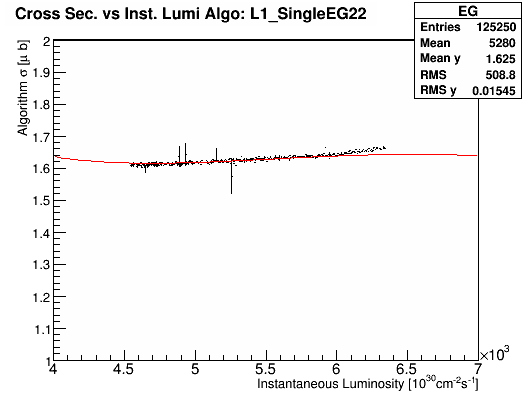
\includegraphics[width=0.45\textwidth]{Chapter03/L1TOnline/Images/L1TDQM_Online_Run207269_L1TRate_TriggerCrossSections_EG.png}
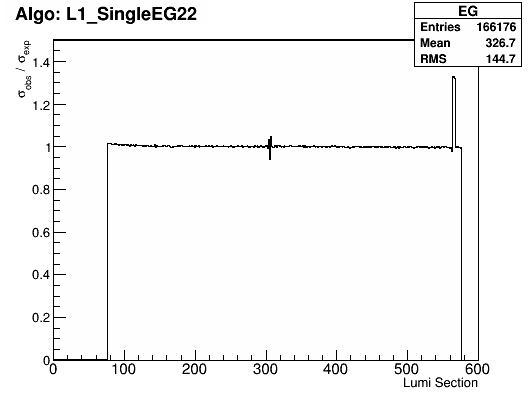
\includegraphics[width=0.45\textwidth]{Chapter03/L1TOnline/Images/L1TDQM_Online_Run207269_L1TRate_Certification_EG.png}
\caption{Monitoring plots produced by the \gls{L1T} online rates monitoring tool for run 207269 and the Electron-Gamma object category. The automatically selected algorithm was L1\_SingleEG22 for this run. On the left histogram the the algorithm cross section as a function of instantaneous luminosity is plotted. The red line is the prediction from fitting data from previous runs while the black points are the measurements for this run. On the right histogram the fraction of the measured value to the prediction is showed for each luminosity section.}
\label{FIGURE:TechnicalWork_RateMonitoring}
\end{figure}

Automatic tests are configured to monitor the produced histograms and flag as bad luminosity sections that show deviation from prediction above 20\%. Marking a specific luminosity section as bad does not invalidate automatically its use for physics analysis but references it for further investigation by the \gls{CMS} shift crew or certification experts.

%%%%%%%%%%%%%%%%%%%%%%%%%%%%%%%%%%%%%%%%%%%%%%%%%%%%%%%%%%%%%%%%%%%%%%%%%%%%%%%%%%%%%%%
%%% SUBSECTION
%%%%%%%%%%%%%%%%%%%%%%%%%%%%%%%%%%%%%%%%%%%%%%%%%%%%%%%%%%%%%%%%%%%%%%%%%%%%%%%%%%%%%%%
\subsection{Synchronization Monitoring}
\label{SECTION:TechnicalWork_L1TDQM_SynchronizationMonitoring}

%Status: DONE

The synchronization monitoring tool has the objective of assessing if each \gls{L1T} object category is being produced and associated with the correct bunch crossing. Similarly to the \gls{L1T} rates monitoring tool described in the previous section, in the beginning of each run we select for each object category the lowest thresholds unprescaled algorithm if available. If none are available the algorithm with lowest prescale and lowest threshold is selected.

The information of which bunch crossings are filled is retrieved at the beginning of each run by \gls{CMS}. That information is stored in a database at point 5 and later replicated to the \gls{CMS} offline conditions database. The synchronization monitoring tool also at the beginning of each run determines the \gls{LHC} fill number from the \gls{L1T} \gls{GT} system which is obtained with the \gls{DIP} directly from the \gls{LHC} control room. With this information the bunch crossing information is retrived from the \gls{OMDS} when running online and from \gls{ORCON} when running offline.

When an events are desynchronized from the correct bunch crossing at the \gls{L1T} level, these events will appear empty from the \gls{HLT} of offline perspectives. Therefore it is unlikely that they will pass any \gls{HLT} triggers making it very difficult to spot this problems. For this reason the synchronization monitoring looks at events that come from special \gls{HLT} trigger, the \gls{HLT} pass-through paths. These triggers are highly prescaled and only required the the a specific \gls{L1T} condition fired. All available \gls{HLT} pass-through paths of single object \gls{L1T} trigger are monitored by this tools.

For each selected event the \gls{GT} records the results of each \gls{L1T} trigger algorithm for the two previous and two posterior bunch crossings. All events triggered by the algorithms selected for monitoring in this five bunch crossing window are compared to the actual \gls{LHC} bunch crossing filling and the results are recorded. Additionally, for each event we query the \gls{GT} about the \gls{LHC} beam mode and if for any event the status is not \text{Stable Beams}, the luminosity section is immediately marked as bad.

Since we are running this monitoring only over the events that pass \gls{HLT} pass-through paths a single luminosity section will typically not have enough statistics to take conclusions on the behaviour of the system. To provide reliable results at the end of each luminosity sections it is decided if the current luminosity section has enough statistics by itself of needs to be grouped with the previous ones. Blocks of luminosity section are made until a minimum number of events is reached for each individual monitored trigger. At this point the histogram of the fraction of events in time with bunch crossings is updated. If the \gls{LHC} beam mode changes or the the run ends, the current open luminosity section block is closed with the current statistics. The histograms produced by this tool for run 207269 can be found in figure \ref{FIGURE:TechnicalWork_SyncMonitoring}.

\begin{figure}[!htb]
\centering
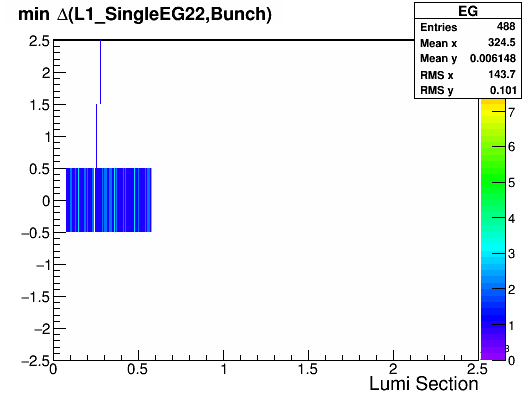
\includegraphics[width=0.45\textwidth]{Chapter03/L1TOnline/Images/L1TDQM_Online_Run207269_L1TSync_AlgoVsBunchStructure_EG.png}
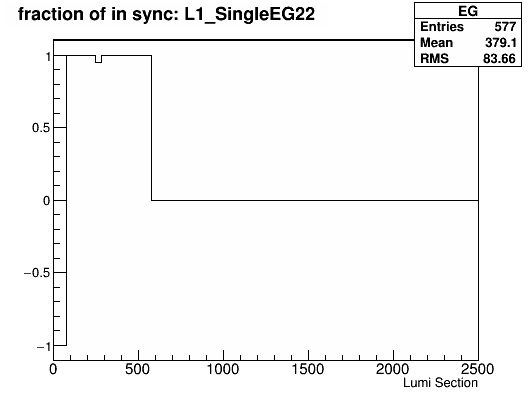
\includegraphics[width=0.45\textwidth]{Chapter03/L1TOnline/Images/L1TDQM_Online_Run207269_L1TSync_Certification_EG.png}
\caption{Monitoring plot produced by the L1TSync tool for L1 single electron/gamma object category, which is
automatically monitoring algorithm L1\_SingleEG22 for the run 207269. In the plots data points are the calculated
trigger cross section as a function of instant luminosity and the line is the reference fit done from previous runs.}
\label{FIGURE:TechnicalWork_SyncMonitoring}
\end{figure}

Similarly to the \gls{L1T} rates monitoring tool, automatic tests are configured to flag as bad luminosity sections that show deviation from prediction above 20\%. 

%%%%%%%%%%%%%%%%%%%%%%%%%%%%%%%%%%%%%%%%%%%%%%%%%%%%%%%%%%%%%%%%%%%%%%%%%%%%%%%%%%%%%%%
%%% SUBSECTION
%%%%%%%%%%%%%%%%%%%%%%%%%%%%%%%%%%%%%%%%%%%%%%%%%%%%%%%%%%%%%%%%%%%%%%%%%%%%%%%%%%%%%%%
\subsection{BPTX Monitoring}

%Status: DONE

The \acrfull{BPTX} system is composed of two beam detectors located in each beam pipe $175\,\meter$ upstream of the \gls{CMS} experiment \cite{ARTICLE:TheCMSExperiment}. This detectors were designed to provide precise information about the bunch structure and timing of each beam and have sensitivity to time structures under $25\,\nano\second$. 

In early 2012 a problem was identified in the \gls{L1T} where some events would fire on the bunch crossing before the actual event. It was discovered the this effect was most likely connect to sensors in the calorimeter system being directly hit by particles causing a large out-of-time signal. Unfortunately, the trigger has a set of rules intended to limit the event rate. They are necessary in order to allow for the necessary latency to extract the information from the detector in case a collision is accepted. One of these rules states that if a collision is accepted by the \gls{L1T} the next 2 collisions are ignore by the system \cite{CMSTDR:CMSTridasTDRVol1}. This means that if a specific event causes the \gls{L1T} to fire on the previous bunch crossing, that event will be vetoed by trigger rules. To avoid losing interesting events due to this pre-firing problem the signal of both \gls{BPTX} detectors logical AND was advanced by one bunch crossing and connected to the trigger via a technical algorithm bit. This bit in turn was used to veto the \gls{L1T} from firing.

Although this was a successful solution to this problem it caused preoccupation in the \gls{TSG} and \gls{L1T} \gls{DPG} groups. Since if the \gls{BPTX} bunch detection threshold would be set too high this veto would be ineffective, leading to no bunches being detect and no veto being applied. If the \gls{BPTX} bunch detection threshold would be set too low, residual amounts of protons or noise in the unfilled bunch spaces could lead to vetoing filled bunch spaces. The development and commissioning of a monitoring tool was requested as priority task.

A new tool was developed to compare the \gls{LHC} filling scheme with the firing of the technical trigger associated with the \gls{L1T}. Following the ideas of the \gls{L1T} synchronization monitoring tool the same procedure was used to retrieve the \gls{LHC} filling scheme and algorithm firing results. In this case we are interested in both efficiency, since low efficiency would mean that the \gls{BPTX} bunch detection threshold would be too low. And miss fire rate, which would be associated with a \gls{BPTX} bunch detection threshold would being too high. Examples of the histograms produced by this tool can be found in figure \ref{FIGURE:TechnicalWork_BPTXMonitoring}.

\begin{figure}[!htb]
\centering
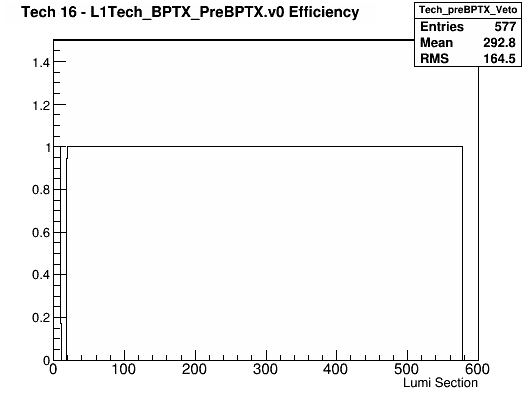
\includegraphics[width=0.45\textwidth]{Chapter03/L1TOnline/Images/L1TDQM_Online_Run207269_L1TBPTX_Efficiency_Tech_preBPTX_Veto.png}
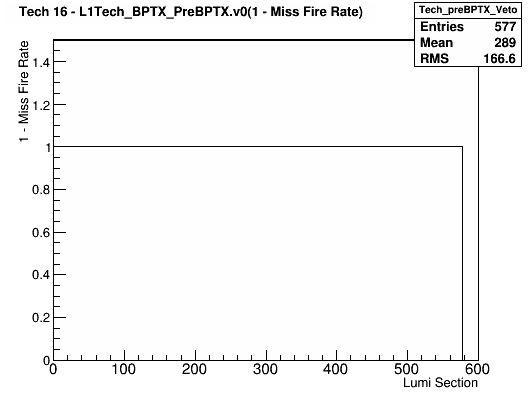
\includegraphics[width=0.45\textwidth]{Chapter03/L1TOnline/Images/L1TDQM_Online_Run207269_L1TBPTX_MissFire_Tech_preBPTX_Veto.png}
\caption{Monitoring plot produced by the \gls{L1T} \gls{BPTX} monitoring tool for \gls{CMS} run 207269. On the left the \gls{BPTX} veto efficiency in relation to the \gls{LHC} fill bunch structure is showed. On the right for the same algorithm $1 - \text{Miss Fire fraction}$ is showed.}
\label{FIGURE:TechnicalWork_BPTXMonitoring}
\end{figure}

%%%%%%%%%%%%%%%%%%%%%%%%%%%%%%%%%%%%%%%%%%%%%%%%%%%%%%%%%%%%%%%%%%%%%%%%%%%%%%%%%%%%%%%
%%% SUBSUBSECTION
%%%%%%%%%%%%%%%%%%%%%%%%%%%%%%%%%%%%%%%%%%%%%%%%%%%%%%%%%%%%%%%%%%%%%%%%%%%%%%%%%%%%%%%
\subsubsection{Implementation Tests}

%Status: DONE

To test that the \gls{BPTX} monitoring tool would be successful in detecting failure of the \gls{BPTX} system a field test was necessary. During run 207269 in which real data recorded the author with the permission of the \gls{L1T} \gls{DPG} disabled the technical \gls{L1T} bit associated with to the \gls{BPTX} AND advanced by one luminosity section which was configured as a veto in the system. The bit was kept disable for a few luminosity sections which was promptly identified by the monitoring tool as it can be seen in figure \ref{FIGURE:TechnicalWork_L1TBPTX_ImplementationTests}.

\begin{figure}[!htb]
\centering
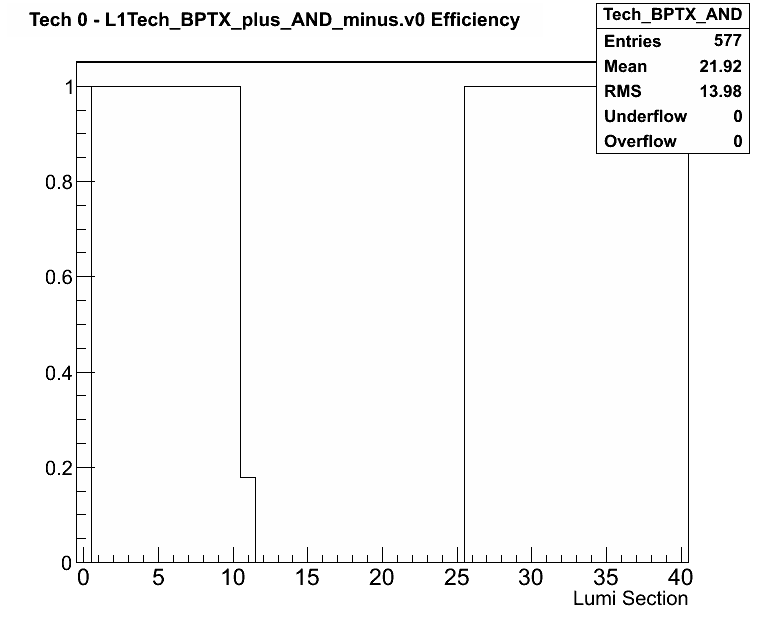
\includegraphics[width=0.45\textwidth]{Chapter03/L1TOnline/Images/L1TBPTX_Tech_BPTX_AND.png}
\caption{Detail of \gls{L1T} \gls{BPTX} monitoring tool histogram for veto efficiency during its field test at run 207269. The monitored bit was disabled manually leading to the monitored drop off efficiency.} 
\label{FIGURE:TechnicalWork_L1TBPTX_ImplementationTests}
\end{figure}

After this successful test the trigger shifter instruction were updated to include this histogram in the periodic checks to be done.  

%%%%%%%%%%%%%%%%%%%%%%%%%%%%%%%%%%%%%%%%%%%%%%%%%%%%%%%%%%%%%%%%%%%%%%%%%%%%%%%%%%%%%%%
%%% SUBSECTION
%%%%%%%%%%%%%%%%%%%%%%%%%%%%%%%%%%%%%%%%%%%%%%%%%%%%%%%%%%%%%%%%%%%%%%%%%%%%%%%%%%%%%%%
\subsection{Occupancy Monitoring}

%Status: DONE

The occupancy monitoring tools objective is to identify regions of detector where the trigger system response has degraded. A region is considered \textit{dead} if the number measurements is null or its rate is consistently smaller than expected for that area. Alternatively, a region can become \textit{hot} if the number of measurements rate is consistently bigger than expected for that area. This tool aims at identifying both of these categories of problems by analysis histograms produced by the trigger subsystems.

The main idea behind these tool is to use the $\eta$ and $\phi$ symmetries of the physics processes and experimental design. The collisions in \gls{CMS} happen in the centre of the experiment with beam of the same energy colliding head-on. Additionally, the detector is symmetric to the beam lines transverse plane passing on the collision point and to the beam line itself. Both this factors imply that the response in strip over $\phi$ at constant $\eta$ should be the same on average everywhere and that response should be equivalent in a similar strip and constant $-\eta$.

The test consists of initially selecting a histogram of a quantity that is an absolute event count per region and that exhibits the described $\eta$ and $\phi$ symmetries. The histogram is integrated for as many luminosity sections as necessary to have enough statistics for conclusive results. When enough statistics are gathered and starting from the centre, a strip of cells is defined along $\phi$ to one side of that symmetry line. The value of the median of the selected cells is determined. Each cell of the opposing strip is compare to this median with a statistical test tuned to detect significant deviations. If the test is failed, the cell is marked as bad for the period of the histogram integration. We repeat the same procedure reversing the role of both strips. After all cells in the first strip pair is tested we move to the next two strips of cells in increasing $\eta$ and repeat the procedure until all cells in the histogram have been tested. For histograms where the symmetry line fall in the middle of a strip of cell, that strip is tested against itself. The median is used to avoid bias from outliers like the \textit{hot} or \textit{dead} cells we are aiming to identify. 

Cells which are already known to be problematic can be masked from this tool to avoid being always marked as bad and contributing to the calculation of the fraction of problematic cells.

%%%%%%%%%%%%%%%%%%%%%%%%%%%%%%%%%%%%%%%%%%%%%%%%%%%%%%%%%%%%%%%%%%%%%%%%%%%%%%%%%%%%%%%
%%% SUBSUBSECTION
%%%%%%%%%%%%%%%%%%%%%%%%%%%%%%%%%%%%%%%%%%%%%%%%%%%%%%%%%%%%%%%%%%%%%%%%%%%%%%%%%%%%%%%
\subsubsection{Statistical hypotheses test}

Since we are analysing histograms of absolute number of entries, like the location on \gls{L1T} Electron-Gamma candidates, each cell will follow Poisson statistics \cite{BOOK:AppliedStatisticsAndProbabilityforEngineers}. The probability of obtaining in an histogram cell value $x$ when the expected value is $\mu$ is expressed in equation \ref{EQUATION:TechnicalWork_Occupancy_Poisson}.

\begin{equation}
P(x;\mu)=\frac{exp(-\mu) \cdot \mu^{x}}{x!}
\label{EQUATION:TechnicalWork_Occupancy_Poisson}
\end{equation}

The statistical test will evaluate each cell over two hypotheses. The null hypothesis $H_0$, considers that the cell is behaving as expected and that the average number of events is $\mu_0$. The alternative hypothesis $H_1$, proposes that this is a problematic cell with an average number of events of $\mu_1$. We can now define out test statistic $T$ as the log-likelihood ratio of the two hypothesis as defined in equation \ref{EQUATION:TechnicalWork_Occupancy_LogLikelihoodRatio}.

\begin{equation}
T=\ln\frac{P(x,\mu_1)}{P(x,\mu_0)}
\label{EQUATION:TechnicalWork_Occupancy_LogLikelihoodRatio}
\end{equation}

This test statistic on the limit of infinity sample size will be $\chi^2$-distributed. If the test statistic $T$ is above the critical value $T_{\text{crit}}$ we do not reject $H_1$, if is it below $T_{\text{crit}}$ we reject $H_1$. The critical value is set to a choice of confidence level of finding a problematic cell. Confidence level of $99\%$ with a fake rate of $1\%$ were chosen to constrain $T_{\text{crit}}$.

Two tests need to be preformed, for the \textit{dead} and \textit{hot} hypotheses. The relationship between between $\mu_0$ and $\mu_1$ for both tests can be defined as $\mu_1=f \cdot \mu_0$ where $f$ is the factional deviation from $\mu_0$ to flag a cell as bad. For the \textit{dead} cell value $f_{\text{dead}}=0.1$ and $f_{\text{hot}}=2.0$ for \textit{hot} cell.

\begin{figure}[!htb]
\centering
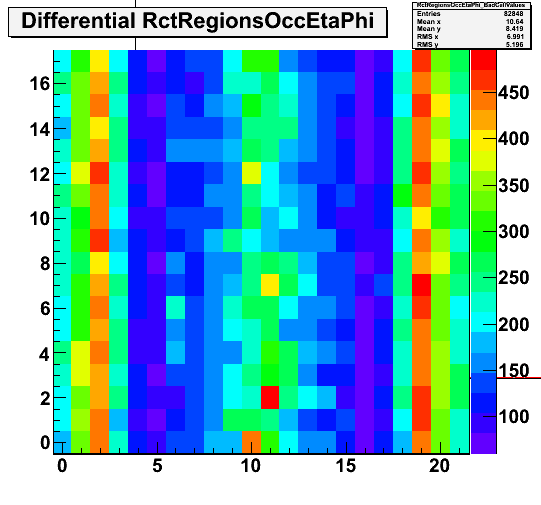
\includegraphics[width=0.45\textwidth]{Chapter03/L1TOnline/Images/L1TOccupancy_Diff.png}
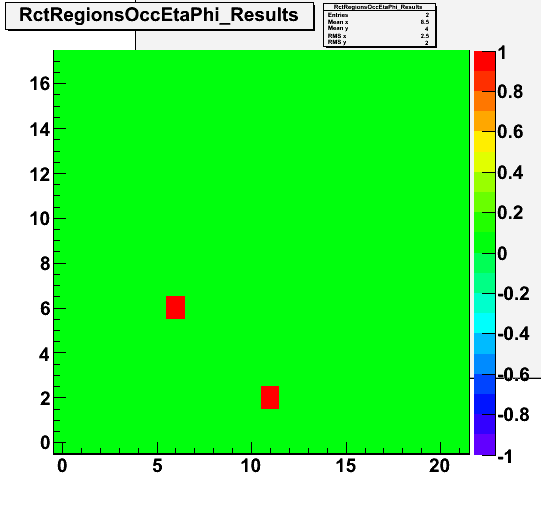
\includegraphics[width=0.45\textwidth]{Chapter03/L1TOnline/Images/L1TOccupancy_Results.png}
\caption{Monitoring plot produced by the L1T Occupancy tool for the run 207099 while testing GCT plot for isolated
EM occupancy $\eta-\phi$. In blue are the masked bins, in green the cells that pass the test and in red the cells
that fail the test. The cells marked as bad are in fact a consequence of the initial plot being produced without
a cut on minimum $p_T$ on the trigger primitives, so the asymmetries observed are due to pedestal differences between
difference areas.}
\label{figure_ServiceWork_L1TOccupancy}
\end{figure}

\section{Tests Summary}

%Status: DONE

To simplify the task of the shift crew and certification for physics analysis an status summary application was developed. This tool collects the results of other tests and presents them in a single set of plots as a function of the luminosity section. Three plots are produced, summaries of the \gls{L1T} rates and \gls{L1T} synchronization monitoring tools, and a global tests summary. On each histogram the bottom horizontal line is a summary which is marked are bad (red) if any of the tests above fails. This scheme allows the user to quickly identify a problem by back tracing information from what tests where marked as bad starting from the summary line on the \textit{L1T Tests Summary} histogram. An example of plots produced by this application can be found in figure \ref{FIGURE:TechnicalWork_TestsSummary}.

\begin{figure}[!htp]%
\centering
\subfloat[]{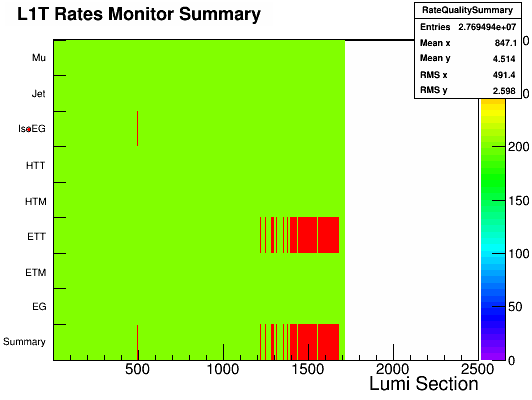
\includegraphics[width=0.45\linewidth]{Chapter03/L1TOnline/Images/RateQualitySummary.png}}\qquad
\subfloat[]{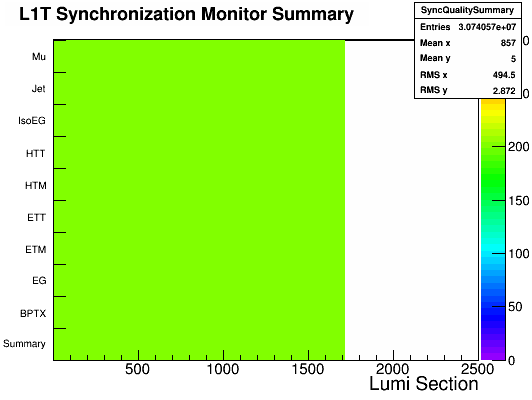
\includegraphics[width=0.45\linewidth]{Chapter03/L1TOnline/Images/SyncQualitySummary.png}}\\
\subfloat[]{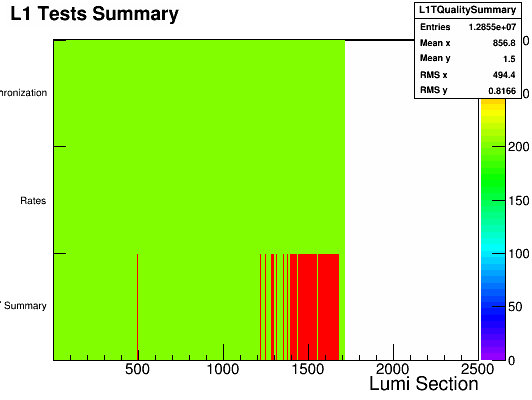
\includegraphics[width=0.45\linewidth]{Chapter03/L1TOnline/Images/L1TQualitySummary.png}}
\caption[Example of the plots produced by the \gls{L1T} test summary monitor]{Example of the plots produced by the \gls{L1T} test summary monitor. Figure (a) the summary of all tests made by \gls{L1T} rates monitor is showed. Figure (b) summary of all tests made by \gls{L1T} synchronization monitor, Figure (c) global summary of all tests performed.}
\label{FIGURE:TechnicalWork_TestsSummary}
\end{figure}

The \gls{L1T} occupancy monitoring was executed over histograms produced by other developers. Some of this histograms suffered from pathological problems that needs intervention from their authors. This caused the summary from that monitoring tool to always be flagged as bad. Although implemented, in order to avoid confusion it was decided to not enable this summary plot or add its results to the global summary until necessary changes to the original histograms were made.

%%%%%%%%%%%%%%%%%%%%%%%%%%%%%%%%%%%%%%%%%%%%%%%%%%%%%%%%%%%%%%%%%%%%%%%%%%%%%%%%%%%%%%%
%%% SECTION
%%%%%%%%%%%%%%%%%%%%%%%%%%%%%%%%%%%%%%%%%%%%%%%%%%%%%%%%%%%%%%%%%%%%%%%%%%%%%%%%%%%%%%%
% \section{Certification}

%Status: Writting

% \section{Proposed Future Upgrades}
